%%%%%%%%%%%%%%%%%%%%%%%%%%%%%%%%%
\newpage
%%%%%%%%%%%%%%%%%%%%%%%%%%%%%%%%%
\section{Shifting squarewave} 

\subsection*{Challenge}
Determine the Fourier series in terms of exponentials and trigonometric terms for the square-wave below and compare it to the square-wave you calculated earlier in challenge \ref{sec:fs_squarewave}. Notice how the presence of the terms are related to the even/odd nature of the function.

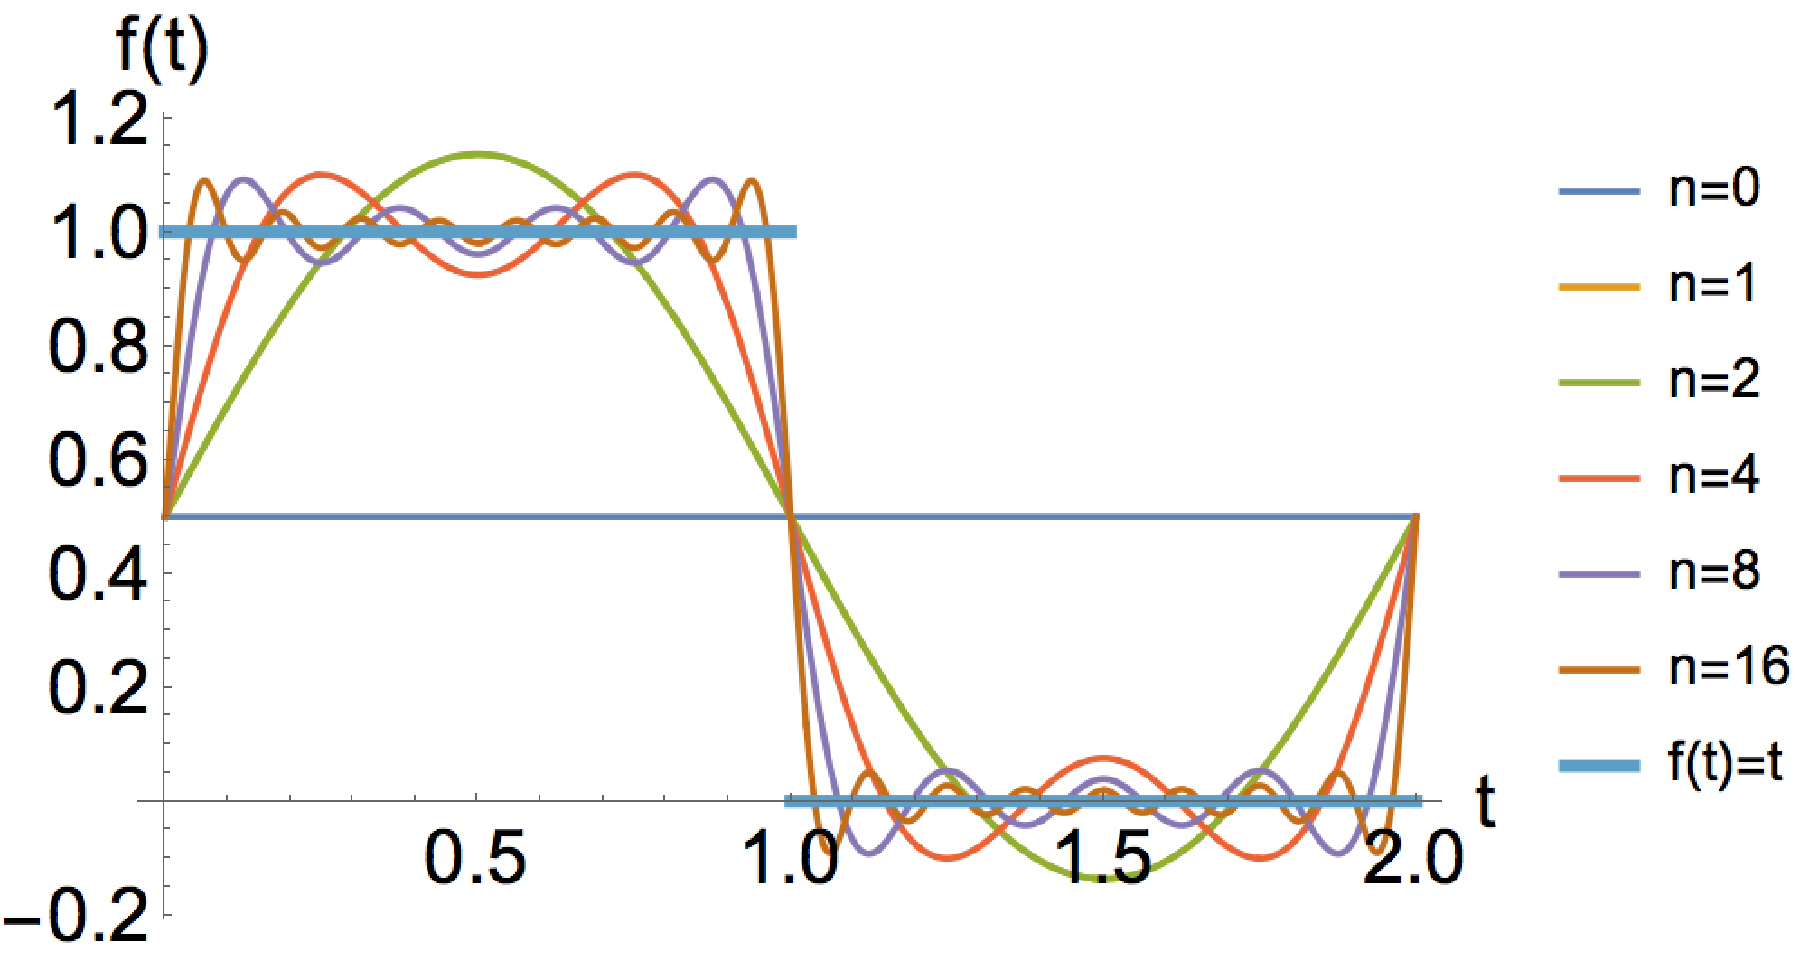
\includegraphics{fs_square_wave_II.png}




%%%%%%%%%%%%%%%%%%%%%%%%%%%%%%%%%
\newpage
%%%%%%%%%%%%%%%%%%%%%%%%%%%%%%%%%
\section{Sawtooth wave} 
\label{sec:sawtooth}

\subsection*{Challenge}
1. Determine the expression for a sawtooth wave of the form shown in the graph below, in terms of a trigonometric Fourier series.

2. Write a sentence explaining how the symmetry of the problem effects the final expression.

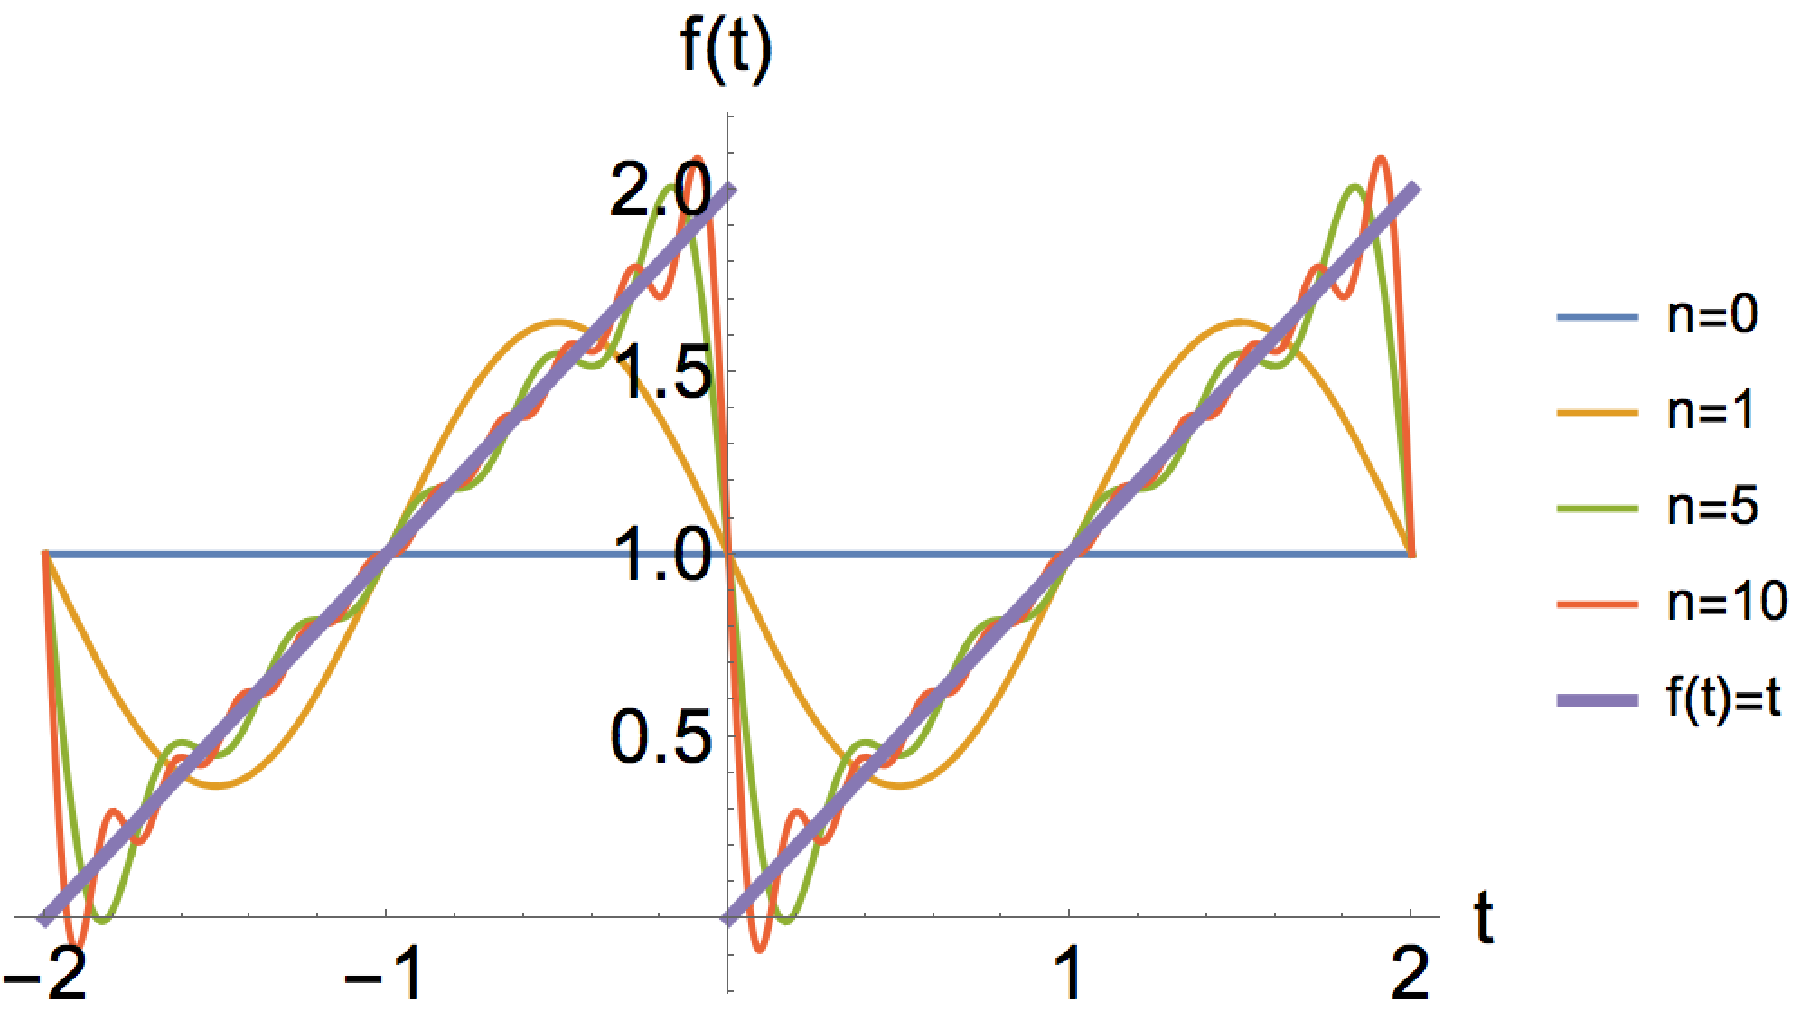
\includegraphics{fs_sawtooth_wave.png}

To check your answer, evaluate the function at $t=1.1$ including only the first 3 terms of the Fourier series.

\subsection*{Solution}
\hash{apaa}{603043}
